%\documentclass[12pt]{report}
%\usepackage{amsmath,graphicx,makeidx}

%\makeindex
%\begin{document}
%\tableofcontents

\chapter{Schematic Creation}
\label{schem}
The first step in the design of an electronic system is the design of its circuit. This circuit is usually created using a {\tt Schematic Editor}\index{Schematic!editor} and is called a {\tt Schematic}. \index{Schematic}Oscad uses {\tt EEschema} \index{EEschema} as its schematic editor. EEschema is the schematic editor of KiCad. It is a powerful schematic editor software. It allows the creation and  modification of components and symbol libraries and supports multiple hierarchical layers of printed circuit design.

\section{Familiarising the schematic editor interface}
Figure \ref{eesch1} shows the schematic editor and the various menu and tool bars. 
\begin{figure}
\begin{center}
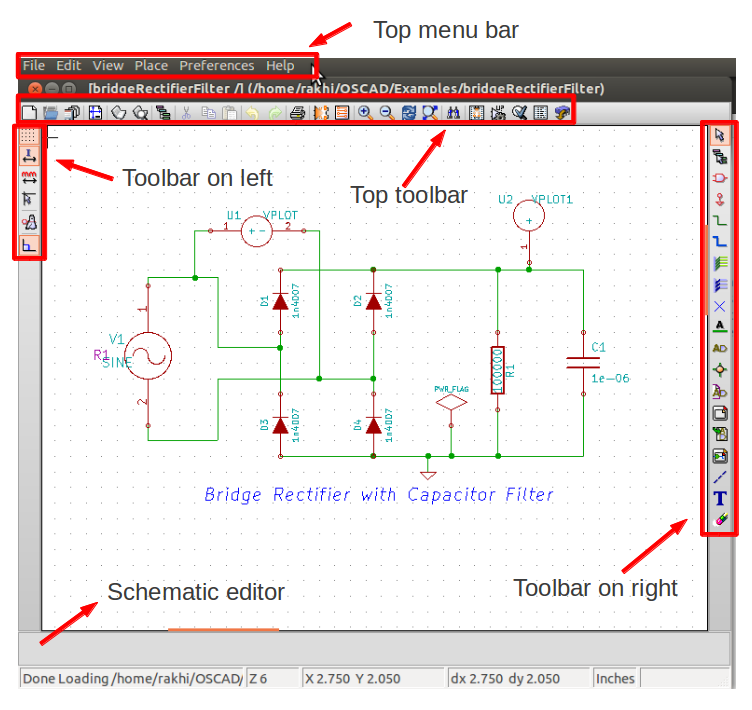
\includegraphics[width=\linewidth]{figures/eeschema1_corctd.png}%If the fig is appearing too big/small, change the scaling factor 0.2
\caption{Schematic editor with the menu and tool bars shown}
\label{eesch1}
\end{center}
\end{figure}



\subsection{Top Menu Bar}
Some of the important menu options in the top menu bar are:
\begin{enumerate}
\item File - 
The file menu items are given below:
\begin{enumerate}
\item New - Clear current schematic and start a new one
\item Open - Open a schematic 
\item Open Recent - A list of recently opened files for loading
\item Save Whole Schematic project - Save current sheet and all its hierarchy.
\item Save Current Sheet Only - Save current sheet, but not others in a hierarchy.
\item Save Current sheet as - Save current sheet with a new name.
\item Print - Access to print menu (See Figure \ref{print}).
\item Plot - Plot the schematic in Postscript, HPGL, SVF or DXF format 
\item Quit - Quit the schematic editor. 
\end{enumerate}
\begin{figure}
\begin{center}
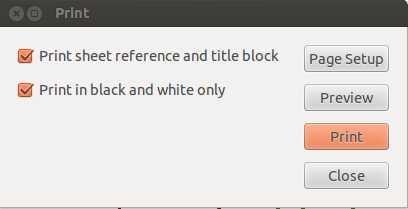
\includegraphics[width=0.5\linewidth]{figures/print.png}%If the fig is appearing too big/small, change the scaling factor 0.2
\caption{Print options}
\label{print}
\end{center}
\end{figure}
\item Place - 
The place menu is a short cut to placing various items like components, wire, junction etc. onto the schematic editor. See the section \ref{short} to know more about various short cut keys (hotkeys).
\item Preferences - 
The preferences menu has the following options:
\begin{enumerate}
\item Library - Select libraries and library paths
\item Colors - Select colors for various items.
\item Options - Display schematic editor options (Units, Grid size).
\item Language - Shows the current list of translations. Use default. 
\item Hotkeys - Access to the hot keys menu. See the section \ref{short} about hotkeys.
\item Read preferences - Read configuration file.
\item Save preferences - Save configuration file.
\end{enumerate}

\end{enumerate} 

\subsection{Top toolbar}\index{Schematic!toolbar!top}
Some of the important tools in the top toolbar are discussed below. They are marked in Figure \ref{eeschem2}
\begin{figure}
\centering
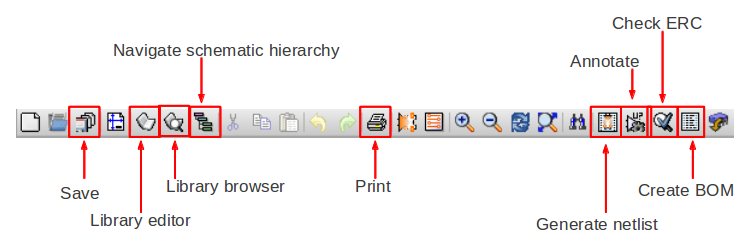
\includegraphics[width=\textwidth]{figures/eeschema2_mod}
\caption{Toolbar on top - important tools}
\label{eeschem2}
\end{figure}
\begin{enumerate}
\item Save - Save your current schematic
\item Library Editor - Create or edit components. See section \ref{component} for more details.
\item Library Browser - Browse through the various component libraries available
\item Navigate schematic hierarchy - Navigate between the root and sub-sheets in the hierarchy
\item Print - Print your schematic
\item Generate netlist - Generate a netlist for PCB design or for simulation.
\item Annotate - Annotate your schematic
\item Check ERC - Do Electric Rules Check for your schematic
\item Create BOM - Create a Bill of Materials of your schematic
\end{enumerate}

\subsection{Toolbar on the right}\index{Schematic!toolbar!right}
The toolbar on the right side of the schematic editor has many important tools. Some of them are marked in Figure \ref{eeschem3}.
\begin{figure}
\centering
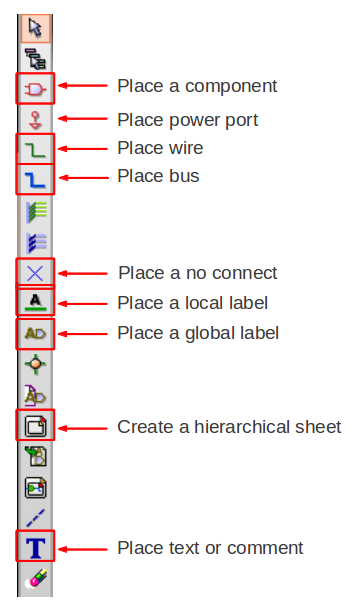
\includegraphics[width=0.6\textwidth]{figures/eeschema3_mod}
\caption{Toolbar on right - important tools}
\label{eeschem3}
\end{figure}

Let us now see these tools one by one.
\begin{enumerate}
\item Place a component - Load a component to your schematic. See section \ref{component} for more details.
\item Place a power port - Load a power port (Vcc, ground) to your schematic
\item Place wire - Draw wires to connect components in schematic
\item Place bus - Place a bus on your schematic
\item Place a no connect - Place a no connect flag, particularly useful in ICs
\item Place a local label - Place a label or node name which is local to the schematic
\item Place a global label - Place a global label (these are connected across all schematic diagrams in the hierarchy)
\item Create a hierarchical sheet - Create a sub-sheet with in the root sheet in the hierarchy. Hierarchical schematics are a good solution for big projects
\item Place a text or comment - Place a text or comment in your schematic
\end{enumerate}
\subsection{Toolbar on the left}\index{Schematic!toolbar!left}
Some of the important tools in the toolbar on the left are discussed below. They are marked in Figure \ref{eeschem4}
\begin{figure}
\centering
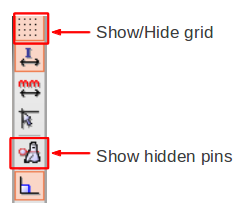
\includegraphics[width=0.5\textwidth]{figures/eeschema4_mod}
\caption{Toolbar on right - important tools}
\label{eeschem4}
\end{figure}

\begin{enumerate}
\item Show/Hide grid - Show or Hide the grid in the schematic editor. Pressing the tool again hides (shows) the grid if it was shown (hidden) earlier.
\item Show hidden pins - Show hidden pins of certain components, for  example, power pins of certain ICs. 
\end{enumerate}

\section{Hotkeys}\index{Hotkeys} 
\label{short}
A set of keyboard keys are associated with various operations in the schematic editor. These keys saves time and make it easy to move from one operation to another. The list of hotkeys can be viewed by going to Preferences in the top menu bar. Choose \textit{Hotkeys} and select \textit{List current keys}. You can also edit the hotkeys by selecting the option \textit{Edit Hotkeys}.
Some of the useful hotkeys are listed below:
\begin{itemize}
\item F1 - Zoom in
\item F2 - Zoom out
\item Ctrl + Z - Undo
\item Delete - Delete item
\item M - Move item
\item C - Copy item
\item A - Add/place component 
\item P - Place power component
\item R - Rotate item
\item X - Mirror component about X axis
\item Y - Mirror component about Y axis
\item E - Edit schematic component
\item W - Place wire
\item T - Add text
\item S - Add sheet
\end{itemize}
\textit{Note that both lower and upper-case keys will work as hotkeys}.
\section{Components and Component libraries}\index{Component}
\label{component}
Oscad schematic editor has a huge collection of components. All the component libraries in EEschema, on which Oscad schematic editor is based, are available. As EEschema is meant to be a schematic editor to create circuits for PCB, EEschema lacks some components that are necessary for simulation (e.g., plots, current sources, etc.). A set of component libraries has been created with such components. 
If you are using Oscad only for designing a PCB, then you might not need these libraries. However, these libraries are essential if you need to simulate your circuit. Hereafter, we will refer to these libraries as \textit{Oscad libraries} to distinguish them from libraries already present in EEschema (EEschema libraries).
\subsection{Oscad libraries}\index{Component!library!Oscad libraries}
The Oscad libraries (created for simulation) are given below:
\begin{enumerate}
\item analogSpice - Discrete components like capacitor, resistor, BJT etc.
\item analogXSpice - Analog Xspice library
\item convergenceAidSpice - To set initial conditions
\item converterSpice - A/D and D/A converters
\item digitalSpice - ICs for digital circuits e.g., the 74 series
\item digitalXSpice - Flip-flops, logic gates etc.
\item linearSpice - 555 timer IC, op amp 741 etc
\item measurementSpice - Plot and print components
\item portSpice - Port
\item sourcesSpice - Current and voltage sources for simulation
\end{enumerate}
Note that the names of all Oscad libraries end with the word \textit{Spice}. Consider the Oscad library \textit{linearSpice}. If you want to simulate a circuit that has a 555 timer IC in it, you should use the 555 timer from this library. This is because only then it will be mapped to the subcircuit of 555 which is required for simulation. Similarly if you use a Flip flop from digitalXSpice, the Xspice description of the Flip flop will be mapped to it and enables us to simulate the Flip flop behaviour.
\subsection{Adding Oscad component libraries to project}
\label{add}
Let us see how you can add the Oscad libraries to your project. Go to \textit{Preferences} from the top menu bar. Choose \textit{Library}. You will get the window shown in Figure \ref{lib}. Click on \textit{Add} (marked in red). Browse to the folder where Oscad is installed. Go to the folder \textit{Library}. Select all the {\tt *.lib} files as shown in Figure \ref{select}. Click on Open. Now click on OK on the window shown in Figure \ref{lib}. 

\textit{Note:} You will have add these to your project each time you create or edit your schematic.

\begin{figure}
\centering
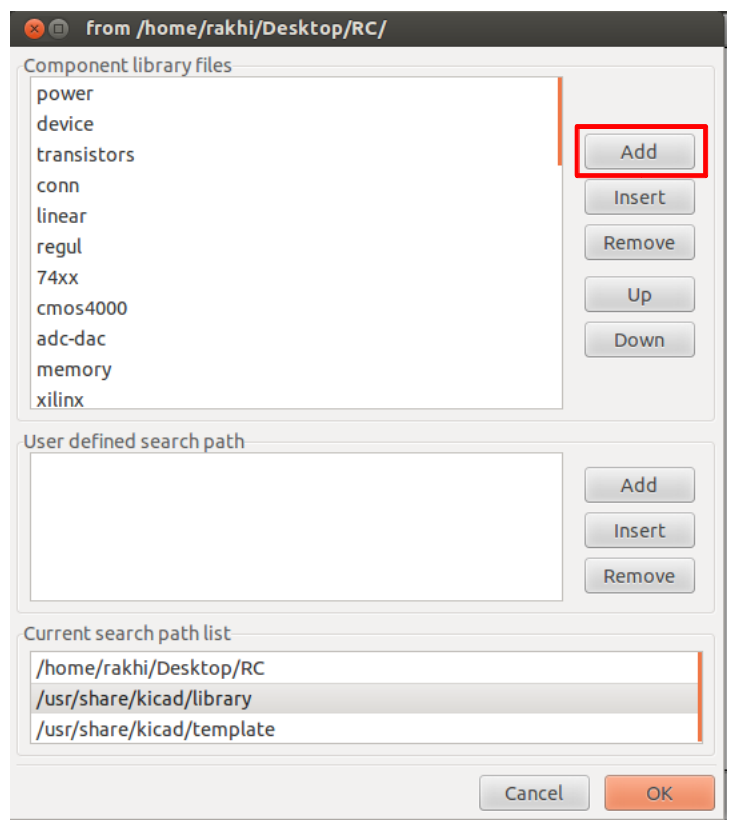
\includegraphics[width=0.65\textwidth]{figures/lib}
\caption{Add component library}
\label{lib}
\end{figure}
\begin{figure}
\centering
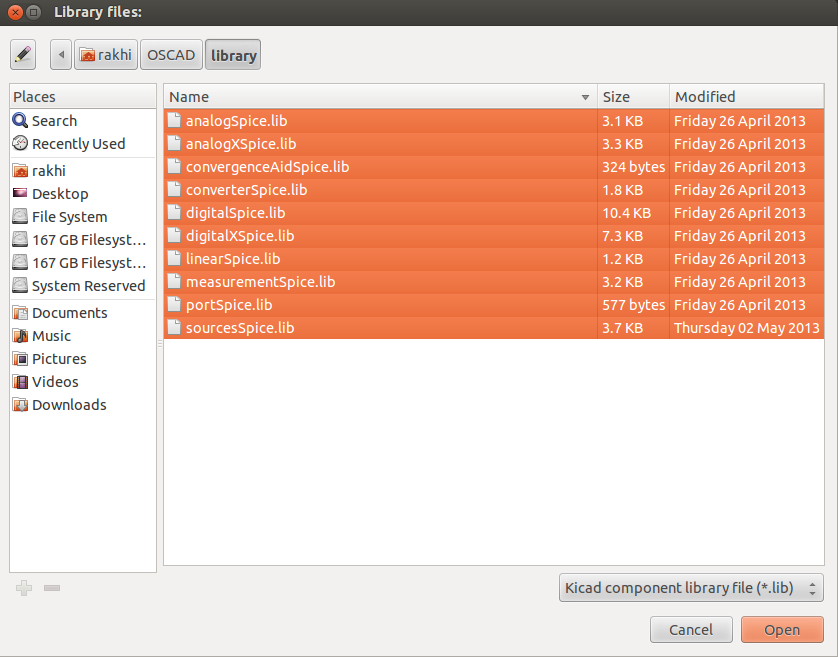
\includegraphics[width=\textwidth]{figures/select}
\caption{Select all the Oscad library (*.lib) files as shown}
\label{select}
\end{figure}
\subsection{Library browser}\index{Component!library}
You can browse through EEschema and Oscad libraries using the library browser tool from the top menu bar. The components in the \textit{sourcesSpice} library is shown in Figure \ref{meas} to illustrate this.
\begin{figure}
\centering
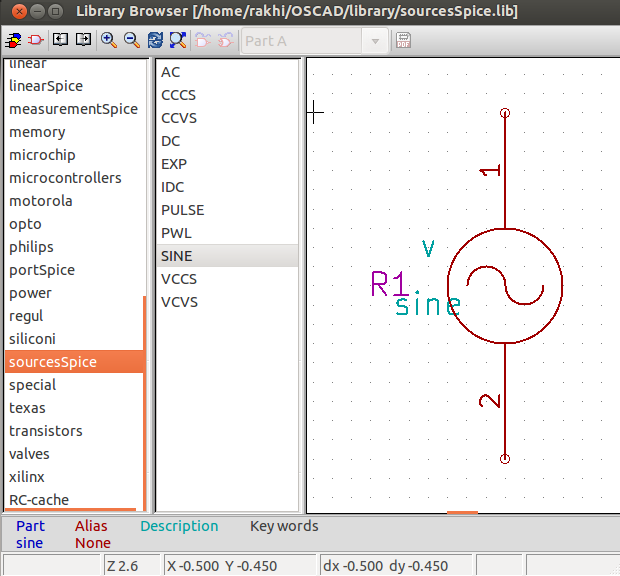
\includegraphics[width=0.7\textwidth]{figures/libbrowse}
\caption{Library browser - an example}
\label{meas}
\end{figure}

\textit{Note that you will be able to view the Oscad libraries in the library browser ONLY IF you have added them to your project as described in Section \ref{add}}
\subsection{Plot component library}\index{Component!library!plot}
Plot components are required to view the results of simulation. These are available in the Oscad library \textit{measurementSpice} shown in Figure \ref{measspice}. These are used only for simulations. Some of the plots available in this library are:
\begin{itemize}
\item IPLOT - Plot the current through a component.
\item VPLOT1 - Plot the voltages at nodes in separate graph windows. 
\item VPLOT8\_1 - Plot the voltages at nodes in the same graph window.
\item VPLOT - Plot the voltage difference between the two nodes where it is placed. 
\begin{figure}
\centering
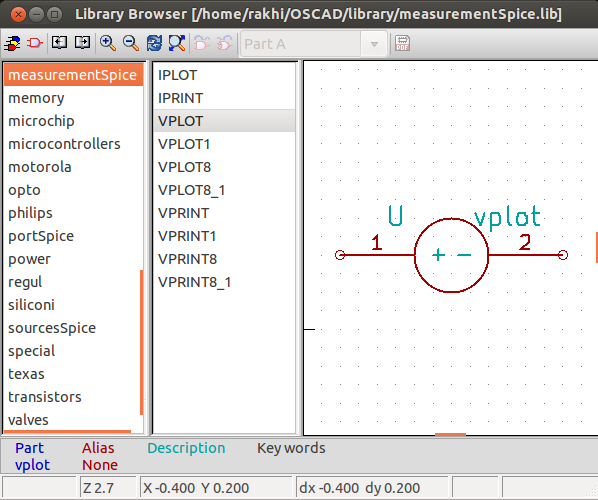
\includegraphics[width=0.6\textwidth]{figures/measspice}
\caption{The Oscad \textit{measurementSpice} library}
\label{measspice}
\end{figure}
\end{itemize}
\subsection{Power component library}\index{Component!library!power}
\label{pwr}
Power components (Vcc and ground) are essential parts of a schematic - both for PCB design and simulation. Power components are available in the EEschema library \textit{power} as shown in Figure \ref{powerlib}. Another important component in this library is the Power Flag, \textit{PWR\_FLAG}. It is a dummy component placed in schematic to tell the schematic editor that the pin/node is driven by a power source and hence prevent ERC errors. 
\begin{figure}
\centering
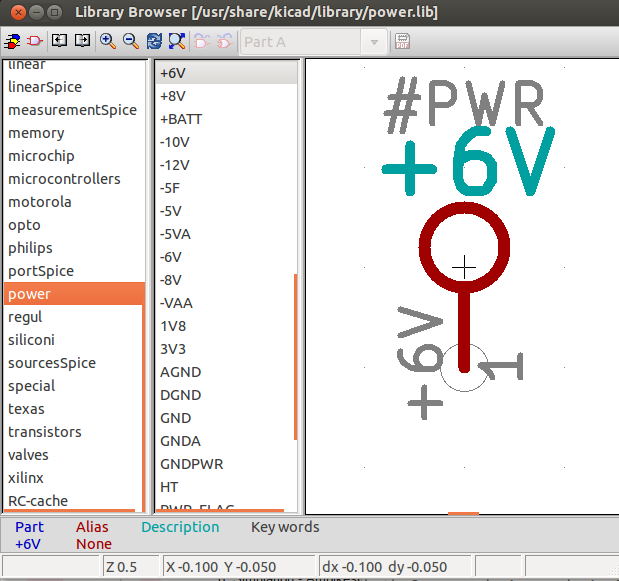
\includegraphics[width=0.7\textwidth]{figures/powerlib}
\caption{The EEschema \textit{power} library}
\label{powerlib}
\end{figure}
\subsection{Connector library}\index{Component!library!connector}
You would want to place connectors in your PCB to take signals in and out of it. These connectors are available in the EEschema library \textit{conn} as shown in Figure \ref{conn}.
\begin{figure}
\centering
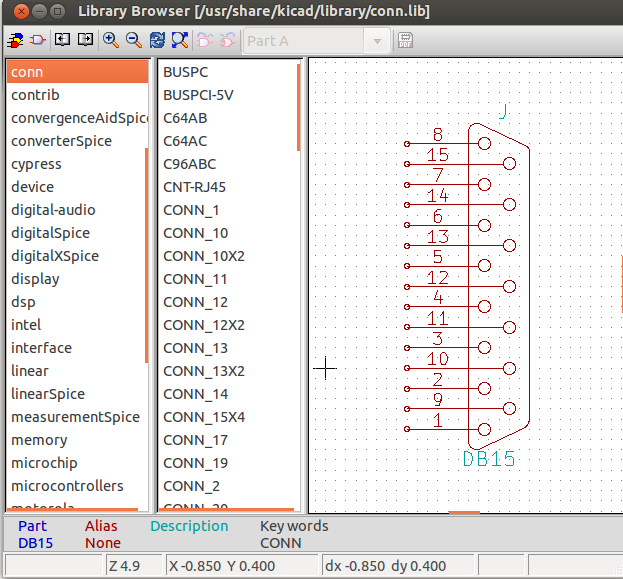
\includegraphics[width=0.6\textwidth]{figures/conn}
\caption{The EEschema \textit{conn} library}
\label{conn}
\end{figure}
\subsection{Component references}\index{Component!reference}
Every component has a unique reference. For e.g., resistor has a reference {\tt R}, BJTs have a reference {\tt Q}, MOSFETs have a reference {\tt M}, ICs have a reference {\tt U} etc. When a component is placed in the schematic editor, the reference will be shown with a question mark. This indicates that the component is not annotated. See section \ref{ann} for more information about annotation.
\section{Schematic creation for Simulation and PCB design - Differences}
There are certain differences between the schematic created for simulation and that created for PCB design. We need certain components like plots, current sources etc. for simulation whereas these are not needed for PCB design. For PCB design, we would require connectors (e.g., DB15, 2 pin connector etc) for taking signals in and out of the PCB whereas these have no meaning in simulation. 
\section{Schematic creation for simulation}
The first step in the creation of circuit schematic is the selection and placement of required components. Let us see this using an example. Let us create the circuit schematic of an RC filter given in Figure \ref{schemRC} and do a transient simulation.
\begin{figure}
\centering
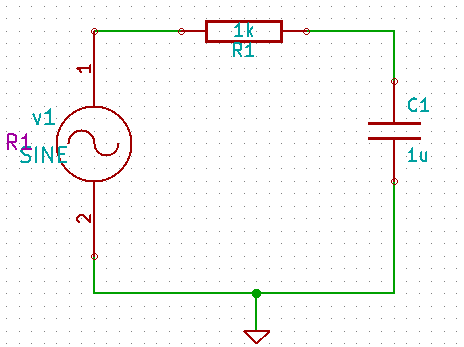
\includegraphics[width=0.35\textwidth]{figures/schemRC}
\caption{RC circuit}
\label{schemRC}
\end{figure}
\subsection{Selection and Placing of components}\index{Component!place}
We would need a resistor, a capacitor, a voltage source, ground terminal and some plot components. 

Add the Oscad libraries to your project as described in section \ref{add}.

To place a resistor on your schematic editor, select the \textit{Place a component} tool from the toolbar on the right side and click anywhere on the schematic editor. This opens up the component selection window. The above action can also be performed by pressing the key A. Type {\tt R} in the field \textit{Name} of the {\tt component selection} window as shown in Figure \ref{res}. Click on OK. A resistor will be tied to the cursor. Place the resistor on the schematic editor by a single click.

\begin{figure}
\centering
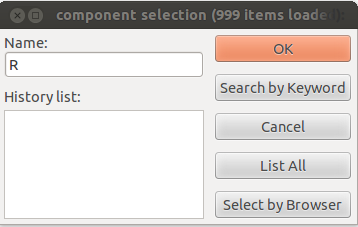
\includegraphics[width=0.5\textwidth]{figures/comp}
\caption{Placing a resistor using the Place a Component tool}
\label{res}
\end{figure}
To place the next component, i.e., capacitor, click again on the schematic editor. Type {\tt C} in the Name field of component selection window. Click on OK. Place the capacitor on the schematic editor by a single click.

Let us now place a sinusoidal voltage source. This is required for performing transient analysis. To place it, click again on the schematic editor. On the component selection window, click on {\tt List all}. Choose the library {\tt sourcesSpice} by double-clicking on it. Select the component {\tt SINE} and click on OK. Place the sine source on the schematic editor by a single click.

We need to place two plot components. Let us place {\tt vplot8\_1} as we need to view input and output waveforms in the same graph window. To do so, choose and place vplot8\_1 from the {\tt measurementSpice} library. To place one more vplot8\_1, place the cursor on top of vplot8\_1 and press the key {\tt C} to copy it. Place the component by clicking on the schematic editor.

Similarly place a ground terminal {\tt gnd} from the library \textit{power}. It can also be placed using the \textit{Place a power port} tool from the toolbar on the right. Click anywhere on the editor after selecting place a power port tool. Click \textit{List all} and choose {\tt gnd}.

Once all the components are placed, the schematic editor would like the Figure \ref{afterplace}.
\begin{figure}
\centering
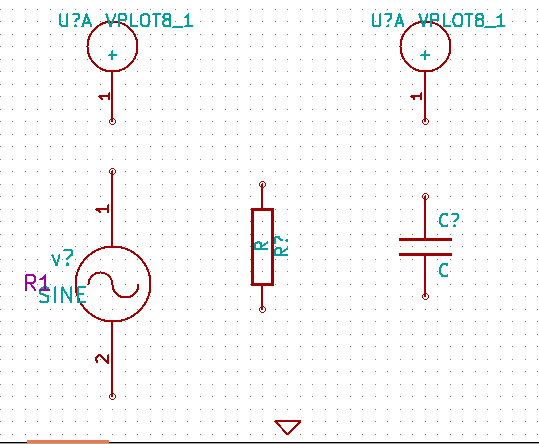
\includegraphics[width=0.5\textwidth]{figures/afterplace}
\caption{All components for RC circuit simulation are placed}
\label{afterplace}
\end{figure}

Let us rotate the resistor to complete the circuit as shown in Figure \ref{schemRC}. To rotate the resistor, place the cursor on the resistor and press the key {\tt R}. Note that if you place the cursor above the letter {\tt R} (not {\tt R?}) on the resistor, you may be asked to clarify selection. Choose the option \textit{Component R}. You can avoid this by placing the cursor slightly away from the letter R as shown in Figure \ref{rotate}. This applies to all components.\index{Component!rotate}
\begin{figure}
\centering
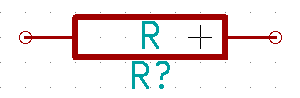
\includegraphics[width=0.3\textwidth]{figures/rotate}
\caption{Place the cursor (shown by the cross mark) slightly away from the letter R}
\label{rotate}
\end{figure}

If you want to move a component, place the cursor on top of the component and press the key {\tt M}. The component will be tied to the cursor and can be moved in any direction. \index{Component!move}
\subsection{Wiring the circuit}
The next step is to wire the connections. Let us connect the resistor to the capacitor. To do so, point the cursor to the terminal of resistor you want to connect and press the key {\tt W}. It has now changed to the wiring mode. Move the cursor towards the terminal of the capacitor and click on it. A wire is formed as shown in Figure \ref{wire1}.
\begin{figure}
\centering
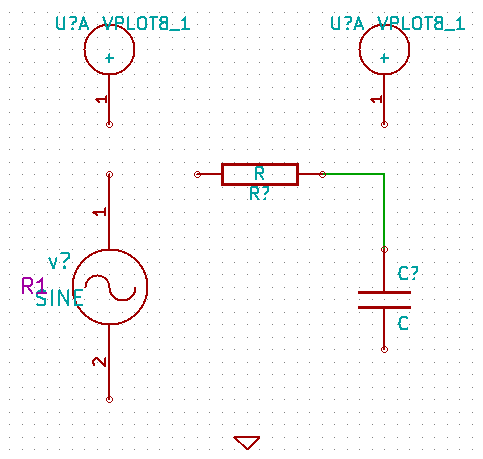
\includegraphics[width=0.5\textwidth]{figures/wire1}
\caption{Wiring example}
\label{wire1}
\end{figure}
Similarly connect the wires between all terminals and the final schematic would look like Figure \ref{wirefin}.
\begin{figure}
\centering
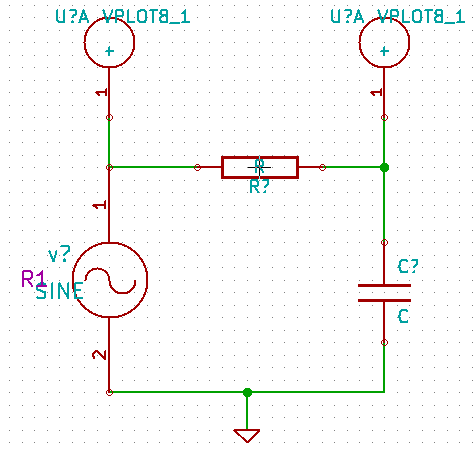
\includegraphics[width=0.5\textwidth]{figures/wirefin}
\caption{Wiring done}
\label{wirefin}
\end{figure}
\subsection{Assigning values to components}\index{Component!values}
We need to assign values to the components in our circuit i.e., resistor and capacitor. Note that the sine voltage source has been placed for simulation. The specifications of sine source will be given during simulation.

To assign value to resistor, place the cursor above the letter {\tt R} (not {\tt R?}) and press the key {\tt E}. Choose \textit{Field value}. Type {\tt 1k} in the \textit{Edit value field} box as shown in Figure \ref{field}. 1k means $1k\Omega$. Similarly give the value {\tt 1u} for the capacitor. 1u means $1\mu F$. 
\begin{figure}
\centering
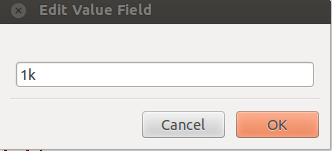
\includegraphics[width=0.5\textwidth]{figures/field}
\caption{Editing value of resistor}
\label{field}
\end{figure}
\subsection{Annotation and ERC}
\label{ann}\index{Annotate}
The next step is to annotate the schematic. Annotation gives unique references to the components. to annotate the schematic, click on \textit{Annotate schematic} tool from the top toolbar. Click on annotate, then click on OK and finally click on close as shown in Figure \ref{anno}. The schematic is now annotated. The question marks next to component references have been replaced by unique numbers. If there are more than one instance of a component (say resistor), the annotation will be done as R1, R2 etc.


\begin{figure}
\centering
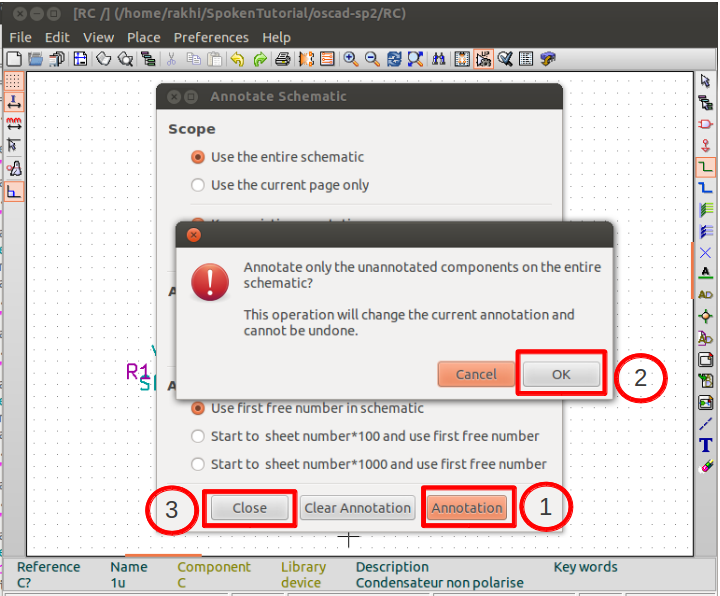
\includegraphics[width=0.78\textwidth]{figures/anno}
\caption{1. First click on Annotate then 2. Click on Ok then 3. Click on close}
\label{anno}
\end{figure}
Let us do ERC or Electric Rules Check next. To do so, click on \textit{Perform electric rules check} tool from the top toolbar. Click on \textit{Test Erc} button. You may get an error as shown in Figure \ref{erc}. Click on close in the test erc window.\index{ERC}
\begin{figure}
\centering
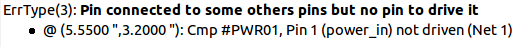
\includegraphics[width=\textwidth]{figures/erc1}
\caption{ERC error}
\label{erc}
\end{figure}
There will be a green arrow pointing to the source of error, here it points to the ground terminal. This is shown in Figure \ref{ercgnd}
\begin{figure}
\centering
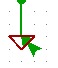
\includegraphics[width=0.1\textwidth]{figures/ercgnd}
\caption{Green arrow pointing to Ground terminal indicating an ERC error}
\label{ercgnd}
\end{figure}

To correct this error, place a {\tt PWR\_FLAG} from the EEschema library {\tt power}. Connect the power flag to the ground terminal as shown in Figure \ref{schemfin}. More information about PWR\_FLAG is given in section \ref{pwr}. Repeat the ERC. Now there are no errors. With this we have created the schematic for simulation.
%\clearpage
\begin{figure}
\centering
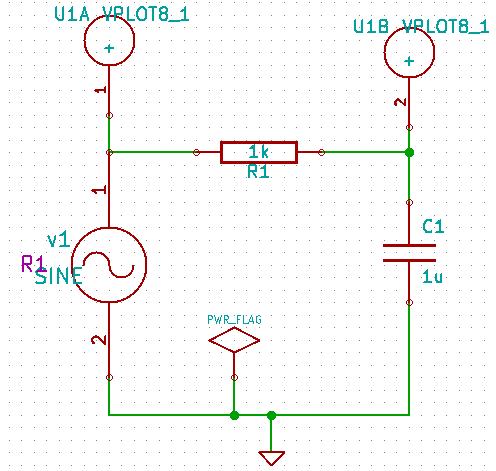
\includegraphics[width=0.5\textwidth]{figures/schemfin}
\caption{Final schematic with PWR\_FLAG}
\label{schemfin}
\end{figure} 
\subsection{Netlist generation}\index{Netlist!for simulation}
To simulate the circuit that you created in the previous section, we need to generate its netlist. {\tt Netlist} is a list of components in the schematic along with their connection information. \index{Netlist} To do so, click on the \textit{Generate netlist} tool from the top toolbar. Click on spice from the window that appears now. Uncheck the option {\tt Prefix references `U' and `IC' with `X'}. Then click on \textit{Netlist}. This is shown in figure \ref{net}. Save the netlist. This will be a {\tt .cir} file. Do not change the directory while saving.
\begin{figure}
\centering
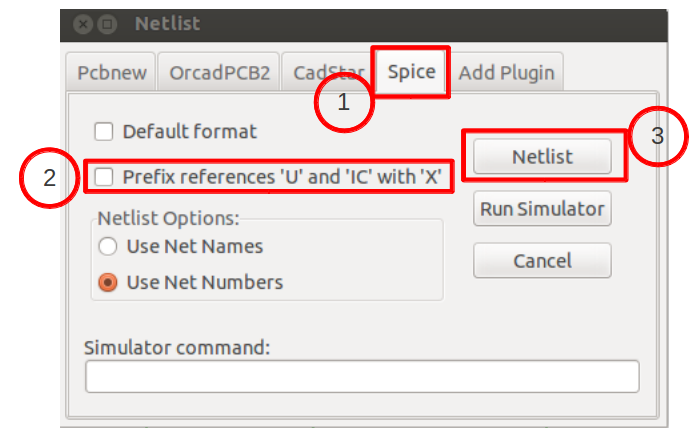
\includegraphics[width=0.5\textwidth]{figures/net}
\caption{1. Click on Spice then 2. Uncheck the option {\tt Prefix references `U' and `IC' with `X'} then 3. Click on Netlist }
\label{net}
\end{figure} 

Now you are ready with the netlist to be simulated. The next chapter will guide you to perform simulation.
%\printindex
%\end{document}
